%% 
%% Copyright 2007-2020 Elsevier Ltd
%% 
%% This file is part of the 'Elsarticle Bundle'.
%% ---------------------------------------------
%% 
%% It may be distributed under the conditions of the LaTeX Project Public
%% License, either version 1.2 of this license or (at your option) any
%% later version.  The latest version of this license is in
%%    http://www.latex-project.org/lppl.txt
%% and version 1.2 or later is part of all distributions of LaTeX
%% version 1999/12/01 or later.
%% 
%% The list of all files belonging to the 'Elsarticle Bundle' is
%% given in the file `manifest.txt'.
%% 

%% Template article for Elsevier's document class `elsarticle'
%% with numbered style bibliographic references
%% SP 2008/03/01
%%
%% 
%%
%% $Id: elsarticle-template-num.tex 190 2020-11-23 11:12:32Z rishi $
%%
%%
\documentclass[preprint,12pt]{elsarticle}

%% Use the option review to obtain double line spacing
%% \documentclass[authoryear,preprint,review,12pt]{elsarticle}

%% Use the options 1p,twocolumn; 3p; 3p,twocolumn; 5p; or 5p,twocolumn
%% for a journal layout:
%% \documentclass[final,1p,times]{elsarticle}
%% \documentclass[final,1p,times,twocolumn]{elsarticle}
%% \documentclass[final,3p,times]{elsarticle}
%% \documentclass[final,3p,times,twocolumn]{elsarticle}
%% \documentclass[final,5p,times]{elsarticle}
%% \documentclass[final,5p,times,twocolumn]{elsarticle}

%% For including figures, graphicx.sty has been loaded in
%% elsarticle.cls. If you prefer to use the old commands
%% please give \usepackage{epsfig}
\usepackage{amssymb}
%% The amsthm package provides extended theorem environments
%% \usepackage{amsthm}

%% The ragged2e package adds text centering
\usepackage[document]{ragged2e}

% use newlines as newlines, instead of \newline
\usepackage{parskip}
\usepackage{xurl}

\journal{Applied Soft Computing}

\begin{document}

\begin{frontmatter}


\title{Multi-objective optimisation of offshore wind farm (OWF) site locations and boundaries in the North Sea}

\author{Zachary Smith}
\affiliation{organization={University of Plymouth},%Department and Organization
            %%addressline={},
            city={Plymouth},
            postcode={PL4}, 
            state={Devon},
            country={England}}

\begin{abstract}
Offshore wind farm site selection is a multi-dimensional problem requiring consideration of spatial and time series data. Due to the volume of data, the use of human agents can be inefficient. This paper explores how genetic algorithms can be well-applied to accelerate this process, formalising expert knowledge into a genetic optimisation problem. We find that social, economic, and engineering constraints can be formalised and used to explore a complex search space, producing solutions that maximise our objectives. We also consider existing installations within our search space and verify the applicability of our research by showing how our algorithm ranks these known solutions.

\end{abstract}

\begin{graphicalabstract}
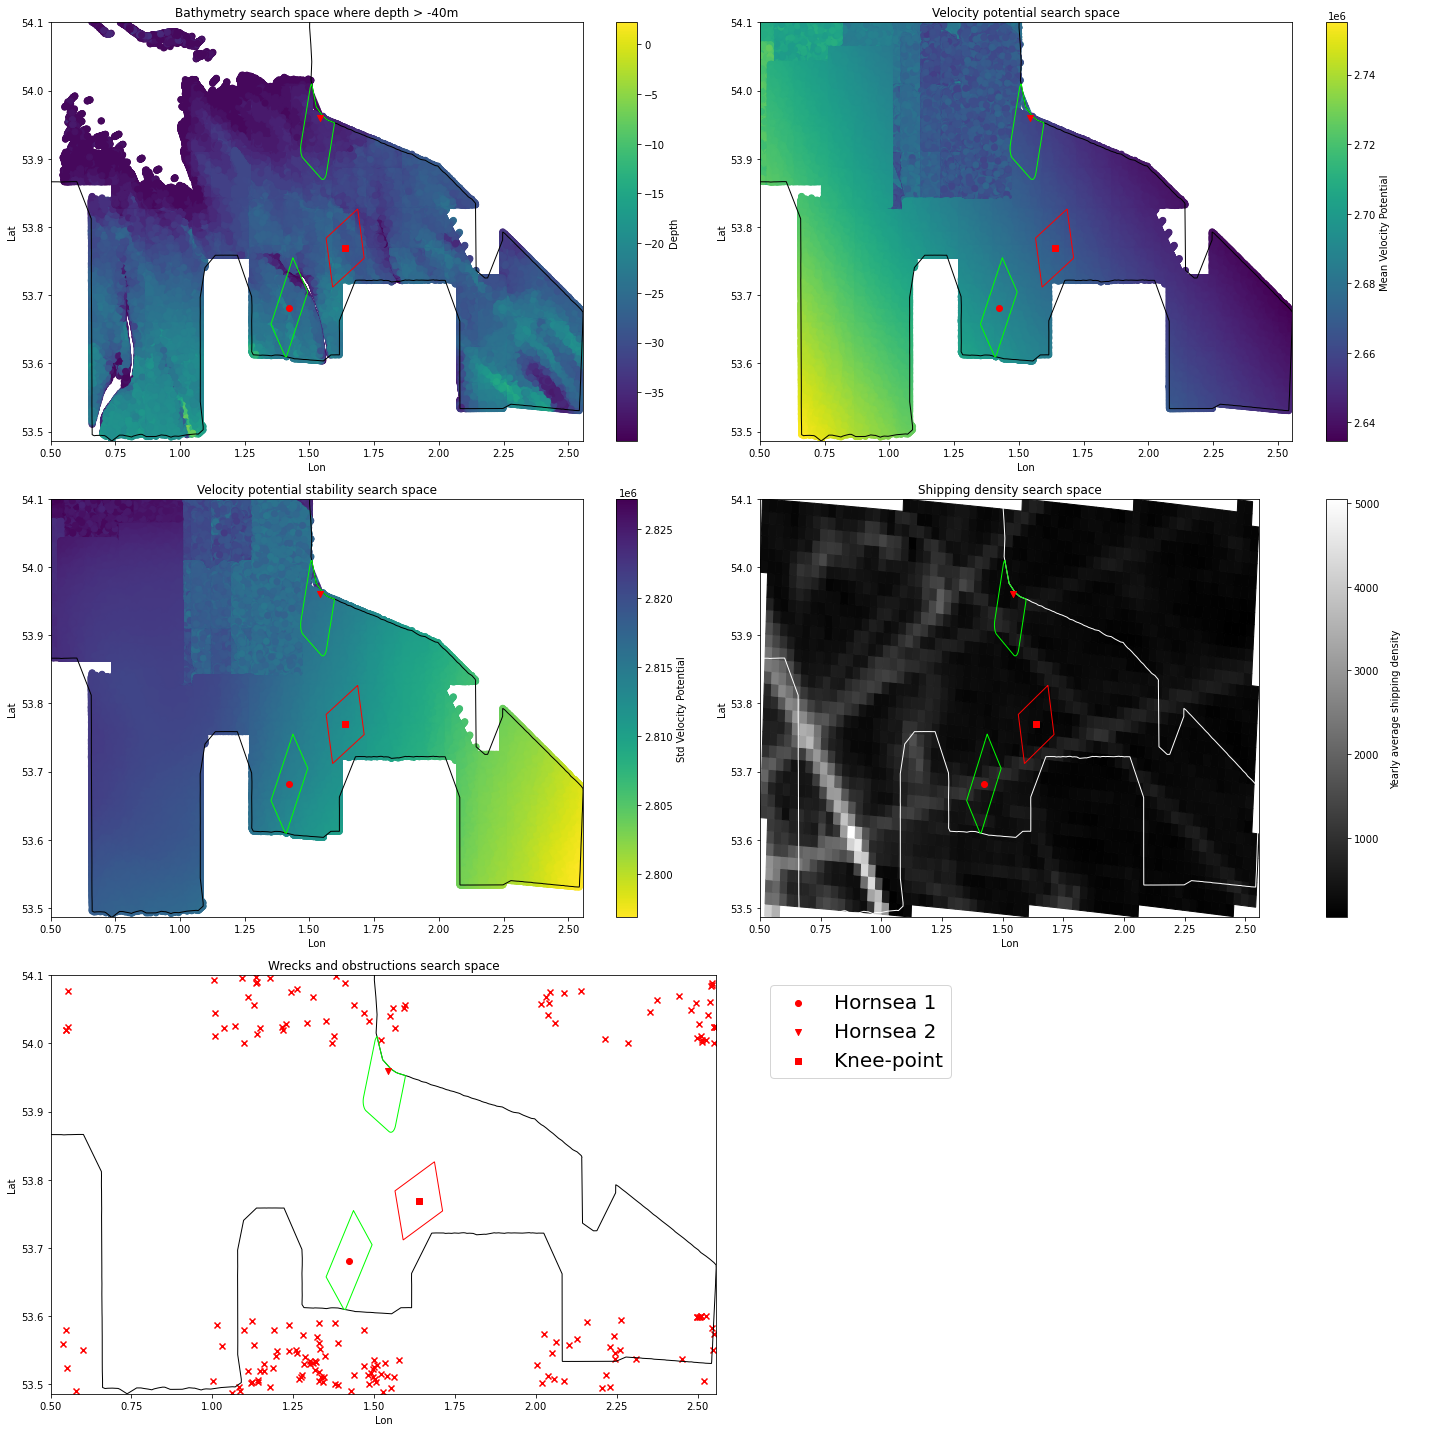
\includegraphics[width=\textwidth,height=\textheight,keepaspectratio]{images/search_space_visualisations.png}
Visualisation of existing Hornsea sites and evolved optimum solution, in the North Sea search space.

\end{graphicalabstract}

%%Research highlights
\begin{highlights}
\item Offshore wind farm site selection is a multi-objective problem with conflicting objectives.
\item Dense neural networks can be used to augment sparse data for performing genetic optimisation.
\item NSGA-III evolves dominant solutions to existing offshore wind farms.
\end{highlights}

\begin{keyword}
%% keywords here, in the form: keyword \sep keyword
Evolutionary Computing \sep Multi-objective Optimisation \sep Power and Energy \sep Process Optimisation
\end{keyword}

\clearpage

\begin{Center}
\textbf{MULTI-OBJECTIVE OPTIMISATION OF OFFSHORE WIND FARM SITE LOCATIONS AND BOUNDARIES IN THE NORTH SEA}

by

\textbf{Zachary Smith}


Thesis submitted to University of Plymouth

in partial fulfilment of the requirements for the degree of


\textbf{\textit{MSc Artificial Intelligence}}


\textbf{University of Plymouth }
\textbf{Faculty of Science \& Engineering}


September 2022
\end{Center}

\vspace*{\fill} %% vertical fill whitespace to move text to bottom of the page
{\raggedleft Elsevier Applied Soft Computing\par}
\clearpage

\textbf{Masters Dissertation licence}:

This material has been deposited in the Plymouth University Learning \& Teaching repository under the terms of the student contract between the students and the Faculty of Science \& Engineering.

The material may be used for internal use only to support learning and teaching.

Materials will not be published outside of the University and any breaches of this licence will be dealt with following the appropriate University policies.

\textbf{Copyright Statement}:

This copy of the thesis has been supplied on condition that anyone who consults it is understood to
recognise that its copyright rests with the author and that no quotation from the thesis and no
information derived from it may be published without the author’s prior written consent.

\clearpage

\textbf{Acknowledgements}:

The author would like to thank their family, partner and friends for their support whilst completing this thesis. 

Special thanks also to Dr David Walker, for supervising the project.

The author would like to acknowledge the National Oceanic and Atmospheric Administration (U.S. Department of Commerce), ADMIRALTY Maritime Data Solutions (U.K. Hydrographic Office), the Marine Management Organisation and the Department for Business, Energy and Industrial Strategy (U.K. Gov) for providing open access to the datasets used in this project.

\clearpage

\end{frontmatter}

%% \linenumbers

%% main text
\section{Introduction}
Electricity production was found to be responsible for 24\% of total greenhouse emissions as of 2013 \cite{Lin2013}. Offshore wind farms (OWFs) are a key component of the U.K.’s commitment to limiting greenhouse emissions and producing electricity domestically through sustainable sources, as part of the Paris Climate Accord to limit global warming.

Maritime spatial planning (MSP) \cite{JAY2010493} is enforced in U.K. waters for projects utilising Crown Estate land. Installation proposals are required to minimise social and environmental impacts in order to be approved. Optimal proposals will maximise energy output and stability whilst conforming to MSP and known engineering constraints.

The Hornsea sites are areas of major investment into offshore renewable energy (ORE) \cite{radov2017offshore}. Hornsea site 1 was the largest OWF at the time of completion \cite{Orsted2018}, superseded only by the completion of Hornsea site 2 \cite{Orsted2022}. With a combined peak output of 2.5GW, the project powers over 2.4 million homes. The scale and impact of this project requires the careful optimisation of several economic, engineering and social factors, contributing to the 10-year timeline for the construction of Hornsea 1. This project is a key example of the need for optimisation of OWF site selection in order to accelerate the construction of ORE projects.

Offshore wind farms are restricted primarily by the availability of shallow water resources, suitable for monopile turbine construction \cite{2019}. It is therefore of primary importance that these finite resources are exploited properly, with proper consideration of the social and economic impacts of the development.

This paper explores the use of nondominated sorting genetic algorithms to optimise this complex search space efficiently. We will develop a multi-dimensional search problem combining numerous engineering, economic and human-impact factors gathered from expert sources, and assess the search space to identify optimal solutions.

\newpage
\section{Methodology}
\subsection{Data collection and analysis}
\begin{figure}[h!]
    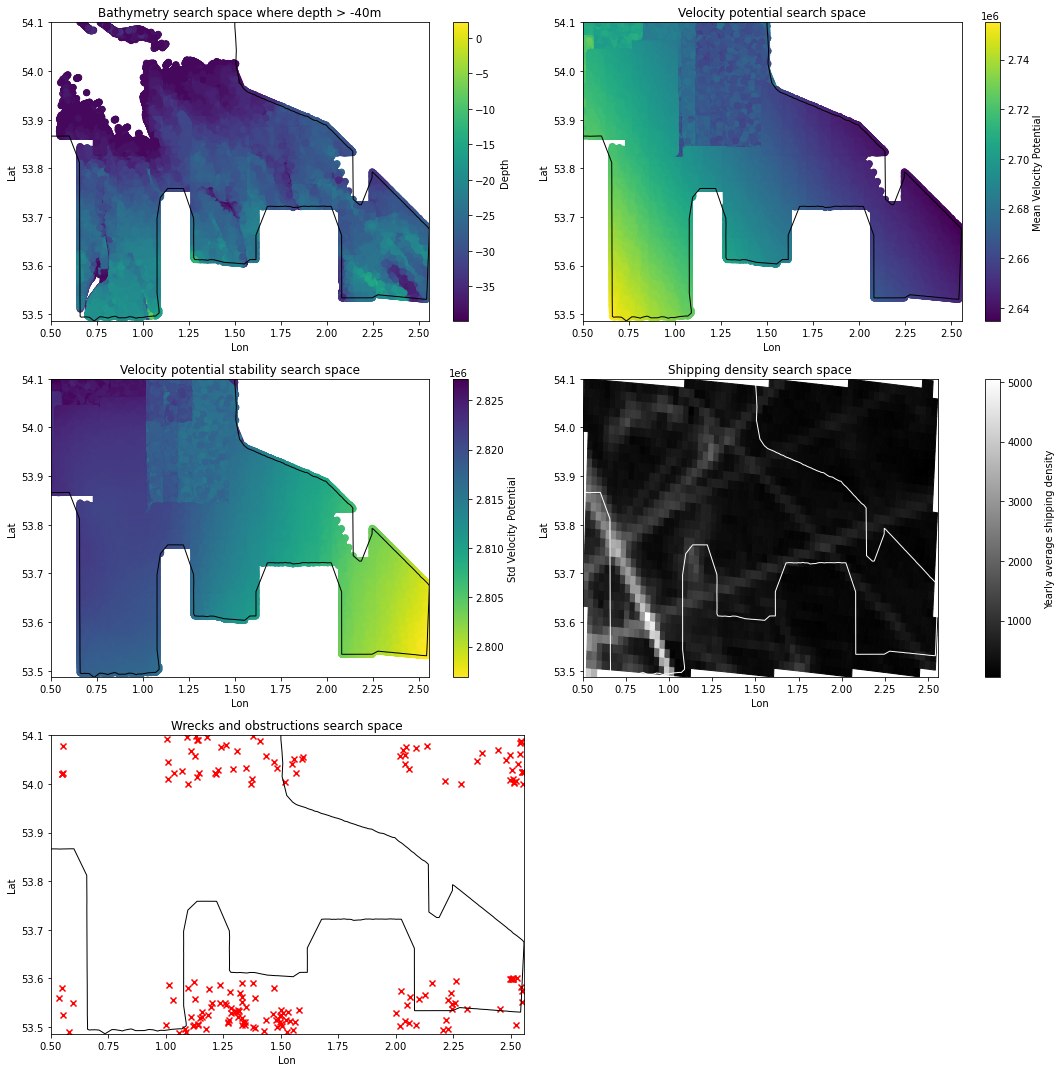
\includegraphics[width=\textwidth,height=\textheight,keepaspectratio]{images/search_space_empty.png}
    \caption{Visualisations of the search space}
    \label{fig:search_space_visualisations}
\end{figure}

To define our search space, we considered relevant criteria used for offshore wind farm site selection in previous studies, finding that criteria generally focussed on engineering feasibility, economic profitability, and impact on human activities. Each category contained objectives to minimise or maximise to generate an ideal solution.

From these objectives, we selected a minimum viable set of objectives to represent the problem, selecting a subset of objectives from each category. We then formalised these objectives into a multi-objective optimisation problem, with the aim of finding a Pareto optimal solution.

We identified six objectives which were common across previous studies: wind energy potential and stability, water depth and presence of obstructions, and shipping activity and distance from shore (figure \ref{fig:search_space_visualisations}). The presence of these objectives in previous studies pre-empts their impact on site location studies, making them viable search spaces to explore with a genetic algorithm \cite{Kim2016}. 

These objectives fell into two categories – hard objectives which had to be met for a solution to be considered feasible, e.g.: maximum water depth, henceforth referred to as constraints, and soft objectives which would be maximised or minimised, often in a trade-off against other soft objectives, e.g.: wind energy and impact on shipping lanes, henceforth referred to as objectives.

Economic objectives concerned the profitability of a potential wind farm. Mean wind velocity and its annual variation are both strong indications of wind turbine performance \cite{punt2009spatial}. Energy output is directly proportional to wind velocity, making it a suitable metric to optimise. The stability of wind velocity is important for maintaining consistent, predictable, power output \cite{NYSERDA2021}, enabling better national grid management, highlighting it as another key objective.

Wind energy and stability data were found to be readily available only as part of a global spatial analysis \cite{2022a}\cite{Kalnay1996}. Time-series spatial data mapped longitude and latitude coordinates to velocity potential, with multiple data points per location covering several months of data. However, it was found that data covering the search space was sparse, leading to a need for data augmentation, as discussed in a later section.

Engineering objectives concerned the interference of the local environment on the site construction. Wreckages and obstructions \cite{hong2011offshore} and water depth \cite{punt2009spatial} were prohibiting factors to construction, due to engineering requirements limiting the maximum depth of turbine monopiles, and associated difficulties or regulations surrounding removing seabed obstructions. Analysing the wreckages and obstructions data, we found numerous wreckages classified as a danger to vessels, highlighting the importance of minimising their inclusion in site boundaries.

Bathymetric depth data was made available as spatial data with irregular sampling \cite{2022b}. As the sampling was sufficiently dense for our search space, and initial testing showed sufficient data could be collected for the minimum area a solution could occupy, this data did not require augmentation.

Social objectives considered the impact of potential farms on existing human activity in that region. We considered minimising the impact on shipping activity to avoid disruption to shipping lanes \cite{kim2010review}. As a part of our search space formulation, we also ensured a minimum of 32km distance from the coast \cite{punt2009spatial}, to reduce noise and visual pollution. We also considered the historical significance of wreckages and sought to minimise or avoid these obstructions as an additional benefit to avoiding engineering complications.

The shipping activity dataset collated GPS data tracking the location of ships into a 2km grid resolution \cite{2017}. This data required minimal pre-processing, and meaningful data could be extracted by estimating the mean shipping density for a site based on the degree of intersection of the site with a given grid square. The wreckages and obstructions dataset \cite{2022} was also relatively clean, with only a small amount of pre-processing required to remove redundant data. As this data was provided in a spatial format, we were able to extract the location of each obstruction and use this to calculate the total number of obstructions per site.

\newpage
\begin{figure}[h!]
    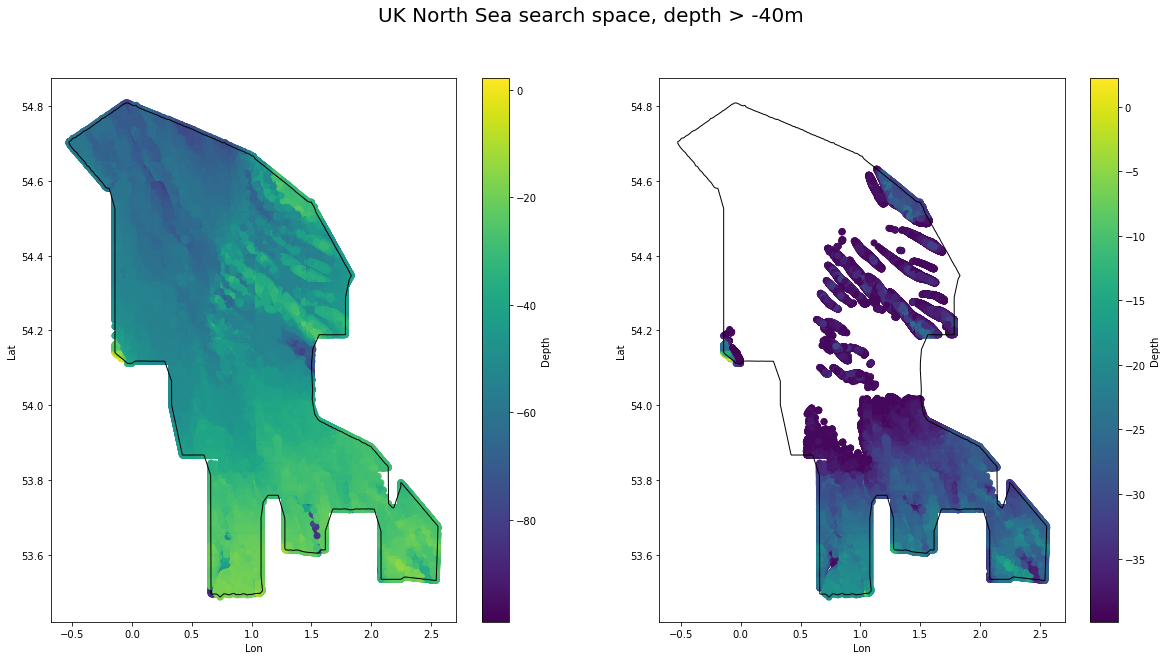
\includegraphics[width=\textwidth,height=\textheight,keepaspectratio]{images/viable_bathymetry.png}
    \caption{Total search space and areas of viable depth.}
    \label{fig:viable_bathymetry}
\end{figure}

Whilst bathymetric data was readily available for some regions, the overlap between these regions of seabed were not regular, as well as some neighbouring regions lacking sample data, meaning we were unable to form a regular search space. Additionally, due to restrictions of the genetic algorithm implementation, solutions could not be explicitly contained to these irregular dimensions. 

In order to ensure solutions were verifiable, an intersection constraint was created to identify feasible solutions. We generated an approximate alpha shape of the search space and used this data to construct a polygon defining the search space boundary (figure \ref{fig:viable_bathymetry}). We could then measure the intersection of solutions with the search space, allowing us to reject out of bounds solutions as infeasible.

We established a maximum viable depth for monopile turbines at -40m, based upon evaluation of the Hornsea sites. However, this depth restriction is arbitrary to our search space, and monopile technology will enable future installations to target deeper sections of the seabed \cite{kallehave2015optimization}. 

Evaluation of the bathymetric data revealed that the initial search space was not entirely viable for turbine installation. The majority of the search space was found to be too deep for turbine installation with these restrictions, with only the Hornsea regions being viable \cite{2019} (figure \ref{fig:viable_bathymetry}). In light of this, the search space was further constrained to only consider these viable regions of seabed.

\subsection{Problem formulation}
In order to define solutions, existing datasets of established offshore wind farm sites were consulted \cite{2022c}. These sites suggested a format for defining our solutions, as well as providing a baseline to validate our model against, based on the assumption existing wind farms will be close to optimal in their search spaces.

Sites were defined spatially using the WGS84 coordinate system \cite{Fell2001} and an indication of the total number of turbines within the site. We estimated the shape of the site assuming turbines were arranged in a typical lattice grid structure and conformed to safety restrictions requiring turbines to be spaced approximately 0.5km apart \cite{SchallenbergRodriguez2018}. This estimated shape formed a minimum site boundary, enabling evaluation of a site assuming turbines occupied this area and exploited the site resources optimially.

Following this format, we defined a genetic code for generating new solutions. Solutions would be defined using a the WGS84 coordinate system,  an optimal number of turbines to define the area of the site, and a rotation in degrees, introduced to enable deeper optimisation of spatially similar sites.

\begin{figure}[h!]
    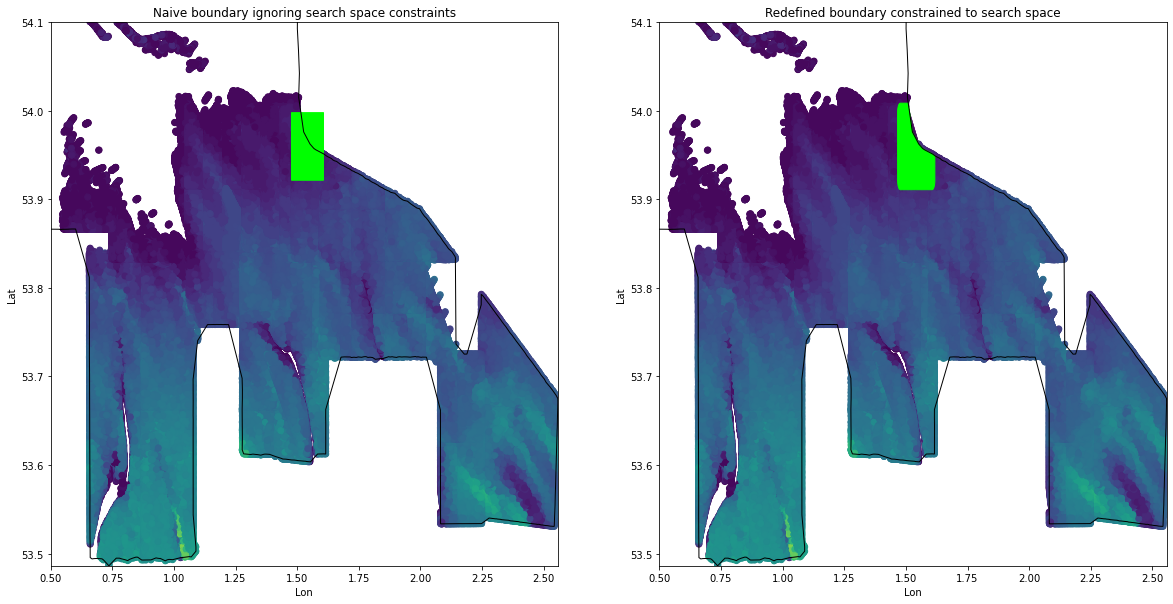
\includegraphics[width=\textwidth,height=\textheight,keepaspectratio]{images/naive_versus_improved_owf_boundary_estimations.png}
    \caption{Comparison of naive and improved algorithms for estimating OWF boundaries.}
    \label{fig:naive_versus_improved_owf_boundary_estimations}
\end{figure}

\newpage
The Hornsea 2 site was found to be located on the edge of our search space, meaning our initial naïve boundary overlapped an unknown space, as observed in figure \ref{fig:naive_versus_improved_owf_boundary_estimations}. Bathymetric data was not publicly available for this region of the seabed, leading us to assume the proper site boundary did not enter this space, requiring us to adjust our method for approximating site boundaries.

Following the assumptions that our estimated site area was correct, the associated spatial coordinates indicated an approximate centre of the site, and that the Hornsea 2 site existed entirely within our search space, we concluded that the true site boundary was an irregular polygon.

In order to approximate this polygon, we calculated the area of disjoint between the naïve shape and the search space and extracted the polygon that intersects the search space. We then buffered the intersecting polygon to redistribute the missing area across the shape, resulting in a new shape with idenical area and less disjoint. Iterating this process allowed us to generate a polygon with the required area, and negligible disjoint with the search space, as shown in figure \ref{fig:naive_versus_improved_owf_boundary_estimations}.

Given our objectives and the solution format, we could consider how to evaluate solutions against our search space. As solutions could be used to create polygons in the search space, and our datasets correlated spatially, we could consider data points based on their inclusion within our site boundary. 

Firstly, wind energy and stability could be summarised for a site based on the mean energy observed across the site over time, whilst stability could be found from the standard deviation of the fluctuations of this energy. Next, water depth constraints could be met by ensuring the depth of the site didn’t exceed the maximum -40m depth, whilst the presence of wrecks and obstructions could be detected through simple bounds checking. Finally, The impact on shipping activity could be estimated by checking the average shipping activity recorded in that sector per week, allowing for areas of increased activity to be avoided.

\newpage
\subsection{Data Augmentation}

\begin{figure}[h!]
    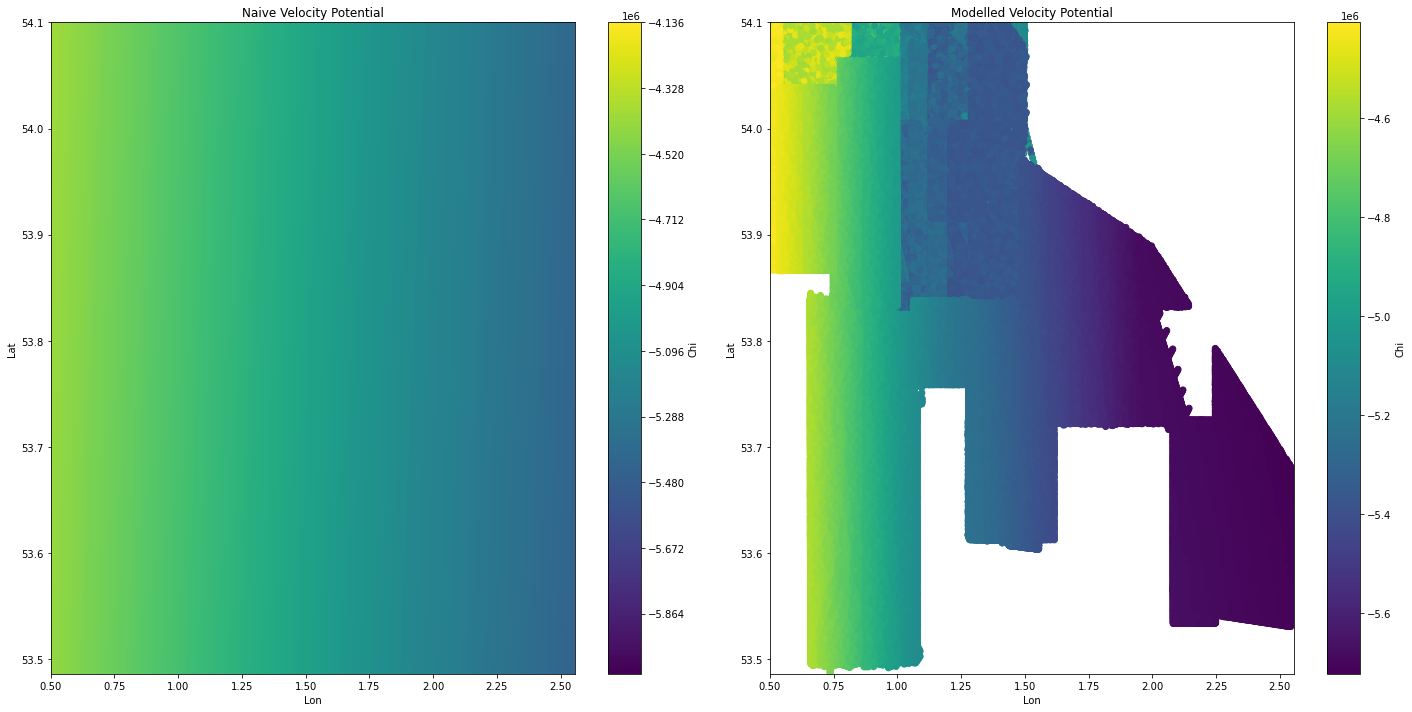
\includegraphics[width=\textwidth,height=\textheight,keepaspectratio]{images/naive_versus_model_velocity_predictions.png}
    \caption{Comparison of naive and deep neural network predictions of velocity potential.}
    \label{fig:naive_versus_model_velocity_predictions}
\end{figure}

As discussed, the wind energy dataset was found to be too sparse to provide data for our search space. We considered two methods of data augmentation to generate a useful dataset. Firstly, we considered the use of interpolation to create linear gradients between known data points. However, this approach resulted in largely homogenous data with no observable features at our desired resolution (figure \ref{fig:naive_versus_model_velocity_predictions}) and extended poorly to a time-series dataset. We, therefore, considered the use of a deep neural network to generate predictions for our search space. We trained a dense model using the known data points as training data and found that the network was able to generate non-homogenous data with observable features. We considered the accuracy of the model by comparing the range of predicted wind energy datapoints within the search space with our interpolated model, finding the models shared a similar range of data, as shown in figure \ref{fig:naive_versus_model_velocity_predictions}. This model allowed us to generate a dataset of predictions to match the resolution of our bathymetric data, which could then be used to evaluate solutions in the search space.

\newpage
\begin{table}[h!]
    \centering
    \begin{tabular}{||c|c|c||}
        \hline
        Layer (type) & Output Shape & Param \# \\
        \hline
        dense\_11 (Dense) & (None, 32) & 128 \\
        \hline
        dense\_12 (Dense) & (None, 64) & 2112 \\
        \hline
        dense\_13 (Dense) & (None, 128) & 8320 \\
        \hline
        dense\_14 (Dense) & (None, 256) & 33024 \\
        \hline
        dense\_15 (Dense) & (None, 512) & 131584 \\
        \hline
        dense\_16 (Dense) & (None, 1024) & 525312 \\
        \hline
        dense\_17 (Dense) & (None, 128) & 131200 \\
        \hline
        dense\_18 (Dense) & (None, 64) & 8256 \\
        \hline
        dense\_19 (Dense) & (None, 8) & 520 \\
        \hline
        dense\_20 (Dense) & (None, 1) & 9 \\
        \hline
    \end{tabular}
    \caption{Model summary (840,465 parameters).}
    \label{table:velocity_model_summary}
\end{table}

The intention behind the model was to accept three inputs – positional longitude/latitude coordinates and a numerical timepoint indicator – and output estimated velocity potential data for that coordinate and timepoint. A 10-layered Dense model was built according to table \ref{table:velocity_model_summary}. Deep learning was specifically considered for this purpose in order to effectively capture spatial features of the dataset and to enable extension into a time-series model. The benefit of a convolutional neural network, as opposed to interpolation, is the preservation of spatial features, and the time-series awareness that enables a more nuanced prediction.

This modelling approach achieved improved resolution for the search space, sufficient for our analysis. Testing with a two-dimensional dataset (without the time-series element) was found to enable better emulation of spatial features, with extension to a third dimension resulting in loss of feature transference, and a more homogenous output. Due to hardware constraints, parameters could not be increased to improve performance, but preliminary results suggest a suitably scaled model could result in more desirable three-dimensional feature transference.

\subsection{NSGA-III}
The Nondominated Sorting Genetic Algorithm III (NSGA-III) \cite{Deb2014} is a popular genetic algorithm used for identifying Pareto fronts of potential solutions for multi-objective search problems. We selected this algorithm due to its improved performance in multi-objective problems versus other popular algorithms such as NSGA-II \cite{deb2000fast} and SPEA \cite{zitzler1999multiobjective}. 

NSGA algorithms work by exploring a search space to identify a population of globally optimal solutions, known as a Pareto front \cite{van1998evolutionary}. Multi-objective problems are often composed of competing or conflicting objectives, meaning multiple solutions can be found that each satisfy some combination of objectives optimally. The establishment of a Pareto front enables the selection of solutions whcih best satisfy requirements through manual weighting of objectives.

The algorithm works by generating an initial population of solutions and evaluating them against the objectives. The population is then iteratively evolved by selecting parents from the population and applying crossover and mutation operators to produce a new population. The new population is then evaluated against the objectives and the process is repeated until a stopping condition is met \cite{Hadka2020}. In our testing, we found that the algorithm was able to identify a Pareto front of solutions within a reasonable number of generations, approximately 5000, with small improvements being observed in subsequent generations past this point.

In order to assess known solutions fairly against evolved solutions, we simulated the evolutionary process while only mutating Hornsea site rotation, keeping site coordinates and number of turbines to static values. We found that the angle of rotation had some impact on site evaluations, producing several solutions that improved slightly upon the naive evaluation. We selected a random solution from this nondominated group to evaluate against evolved solutions.

\newpage
\section{Results and Discussion}
\begin{figure}[h!]
    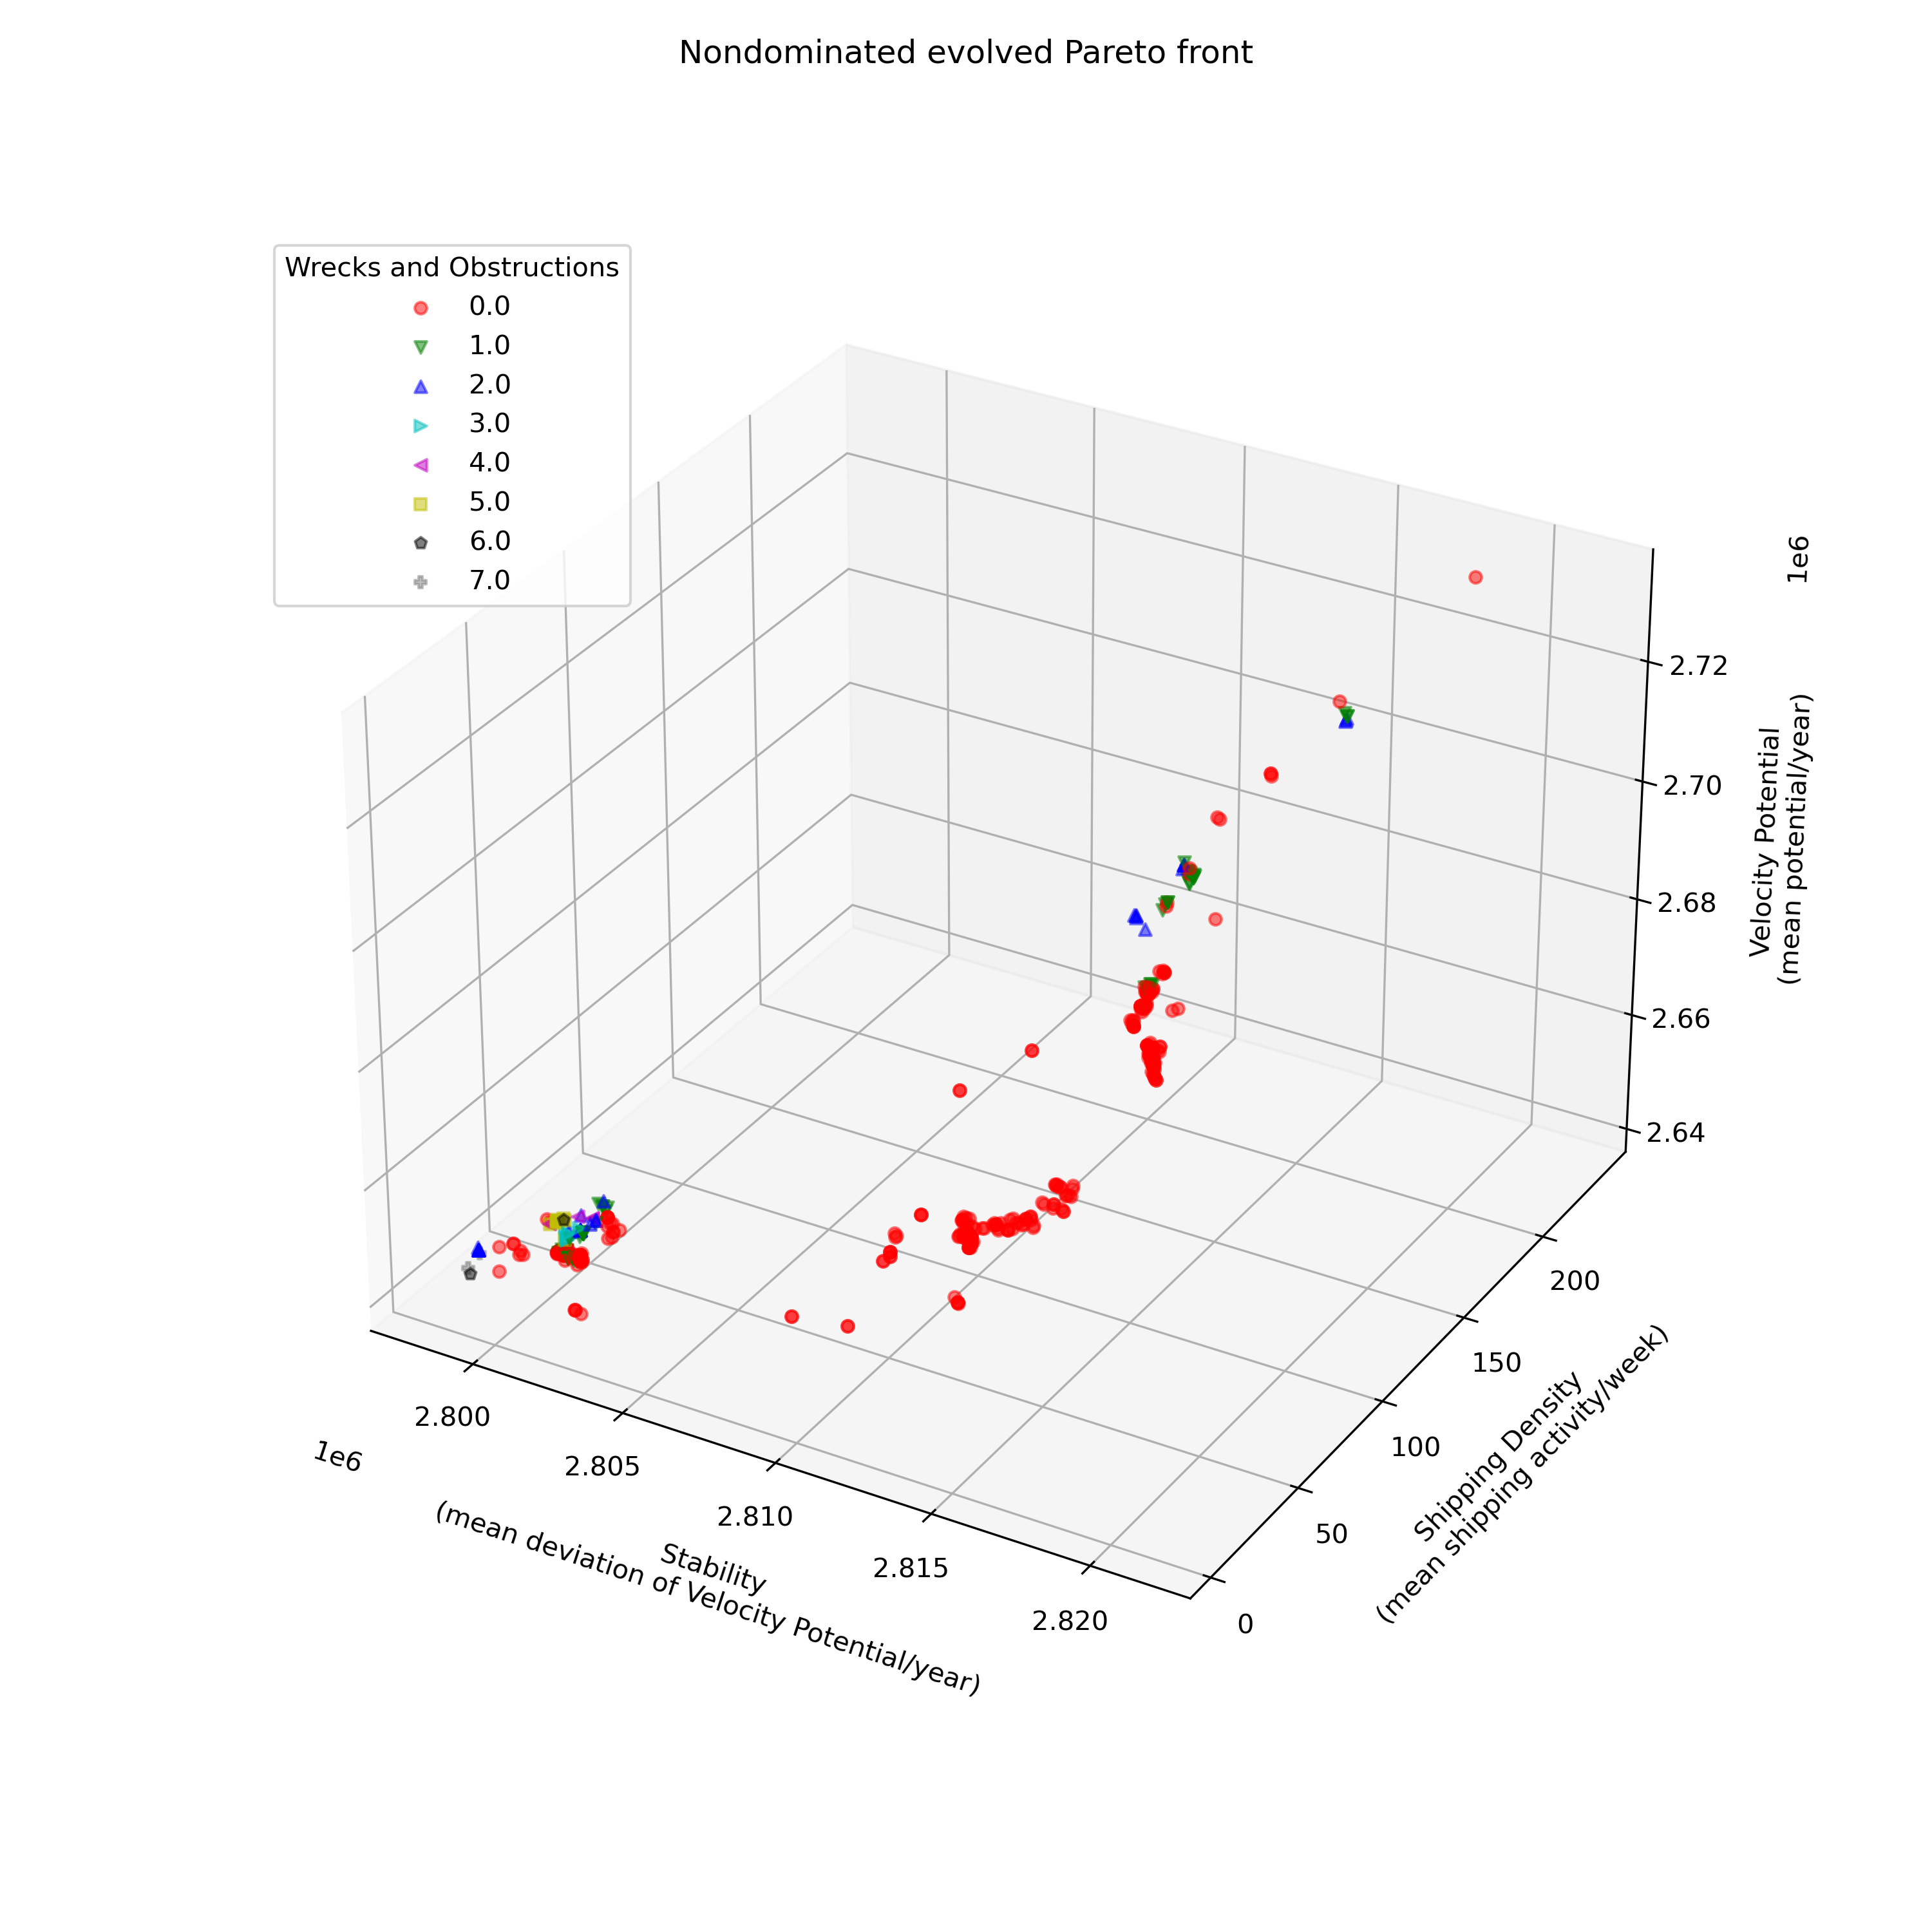
\includegraphics[width=\textwidth,height=\textheight,keepaspectratio]{images/nondominated_evolved_pareto_front.png}
    \caption{Nondominated evolved Pareto front}
    \label{fig:nondominated_evolved_pareto_front}
\end{figure}

From the evolved Pareto front, a multitude of solutions could be selected to balance objectives according to an arbitrary set of weights. In order to compare a single most minimising solution against the Hornsea sites, the knee-point of the Pareto front was found. A knee-point solution on a Pareto front is the point where further improvements in any individual objective would be accompanied by a decrease in another objective, indicating a given solutions optimal nature. This solution is often considered the most optimal solution for a given set of objectives \cite{Maltese2016}.

\begin{table}[h!]
    \centering
    \begin{tabular}{|p{0.9\textwidth}|}
        \hline
        \begin{itemize}
            \item Design variables
            \begin{itemize}
                \item Longitude: 1.646548
                \item Latitude: 53.769962
                \item Rotation: 241.47251°
                \item Turbines: 173
            \end{itemize}
            \item Objectives
            \begin{itemize}
                \item Velocity potential: 2.668589e+06
                \item Velocity potential stability: 2.812422e+06
                \item Shipping density: 7.179781
                \item Wrecks and obstructions: 0
            \end{itemize}
            \item Constraints
            \begin{itemize}
                \item Max. depth of water: -34.9m
            \end{itemize}
        \end{itemize} \\
        \hline
    \end{tabular}
    \caption{Knee-point solution}
    \label{table:kneepoint_solution}
\end{table}

As each objective worked to different scales, the Pareto front must be normalised before selection. We normalised the data using maximum absolute scaling, rescaling each feature between -1 and 1 to retain sign data and proportionality whilst constraining each objective to a common range to remove bias when selecting an optimal solution.

The knee-point solution is shown in table \ref{table:kneepoint_solution}. Iterative testing of the NSGA-III algorithm has produced almost identical knee-point solutions for each run, with only minor differences in the number of turbines and rotation, depending on the number of generations the algorithm was allowed to run. Because of this consensus, we will discuss the knee-point solution as a global optimum of the search space.

\newpage
\begin{table}[h!]
    \centering
    \begin{tabular}{|p{0.9\textwidth}|}
        \hline
        \begin{itemize}
            \item Design variables
            \begin{itemize}
                \item Longitude: 1.422626
                \item Latitude: 53.681258
                \item Rotation: 49.0°
                \item Turbines: 174
            \end{itemize}
            \item Objectives
            \begin{itemize}
                \item Velocity potential: 2.690312e+06
                \item Velocity potential stability: 2.814096e+06
                \item Shipping density: 52.433040
                \item Wrecks and obstructions: 0
            \end{itemize}
            \item Constraints
            \begin{itemize}
                \item Max. depth of water: -17.2m
            \end{itemize}
        \end{itemize} \\
        \hline
    \end{tabular}
    \caption{Hornsea site 1}
    \label{table:hornsea_site_1}
\end{table}

\begin{table}[h!]
    \centering
    \begin{tabular}{|p{0.9\textwidth}|}
        \hline
        \begin{itemize}
            \item Design variables
            \begin{itemize}
                \item Longitude: 1.541901
                \item Latitude: 53.959745
                \item Rotation: 247.0°
                \item Turbines: 165
            \end{itemize}
            \item Objectives
            \begin{itemize}
                \item Velocity potential: 2.662278e+06
                \item Velocity potential stability: 2.815642e+06
                \item Shipping density: 10.534137
                \item Wrecks and obstructions: 1
            \end{itemize}
            \item Constraints
            \begin{itemize}
                \item Max. depth of water: -29.9m
            \end{itemize}
        \end{itemize} \\
        \hline
    \end{tabular}
    \caption{Hornsea site 2}
    \label{table:hornsea_site_2}
\end{table}

Existing data for the Hornsea sites provided only an approximate spatial coordinate and number of turbines used per site. We applied the same evaluation process to this data as we did to our evolved solutions, generating approximate boundaries based on the minimum expected area of the site, finding the sites had evaluations as shown in table \ref{table:hornsea_site_1} and \ref{table:hornsea_site_2}.

\begin{figure}[htp!]
    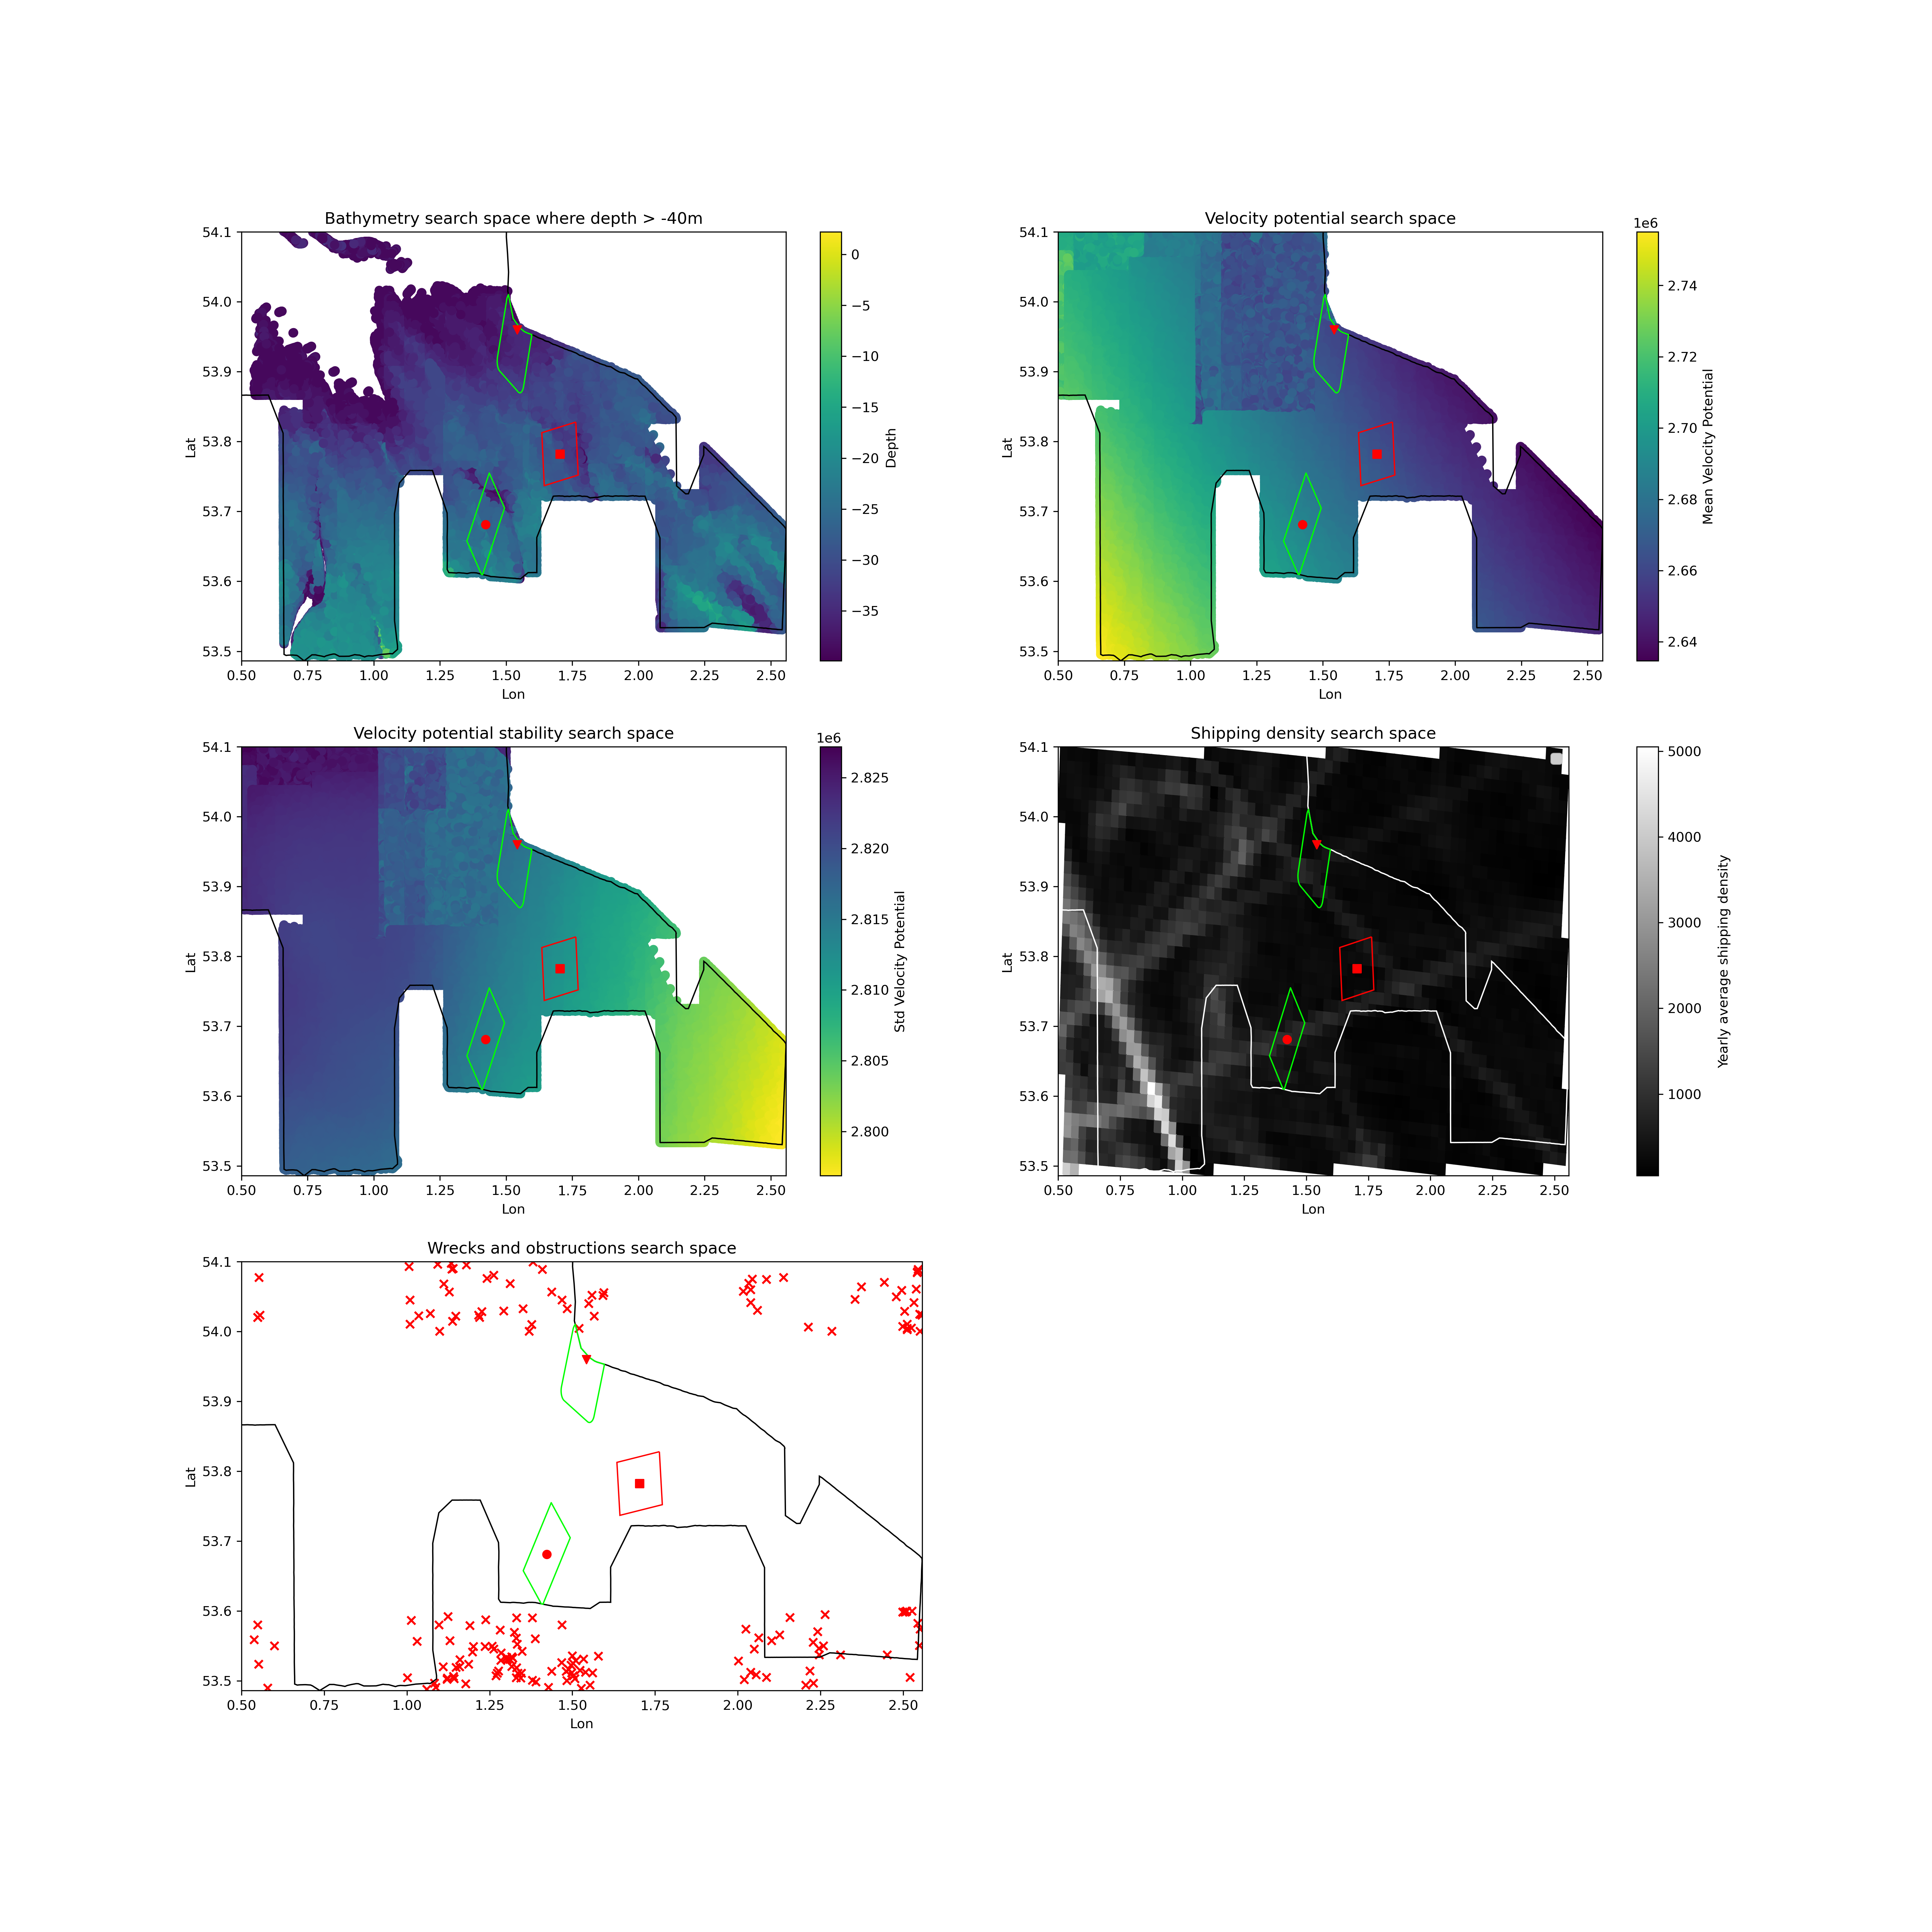
\includegraphics[width=\textwidth,height=\textheight,keepaspectratio]{images/all_results_visualisations.png}
    \caption{Global optima and Hornsea sites visualised in the search space.}
    \label{fig:all_results_visualisations}
\end{figure}

\newpage
\begin{table}[h!]
    \centering
    \begin{tabular}{||c|c|c|c|c||}
        \hline
        Sitename & Velocity potential & Stability & Shipping density & Wrecks and Obstructions \\
        \hline
        Hornsea 1 & -0.75\% & -0.06\% & -86.31\% & 0.0\% \\
        \hline
        Hornsea 2 & -0.24\% & -0.11\% & -31.84\% & -100.0\% \\
        \hline
    \end{tabular}
    \caption{Improvements made by knee-point solutions vs. Hornsea sites; negative values indicate improvements.}
    \label{table:kneepoint_percentage_improvements}
\end{table}

Evaluating these approximate search spaces, we found the Hornsea 1 site was generally dominant against Hornsea 2, and nondominant against the knee-point solution. However, this dominance is largely due to the inclusion of an obstruction within the Hornsea 2 site boundary. Excluding this objective, the Hornsea sites are mutually nondominant.

Comparing the percentage change between Hornsea evaluations and the evolved solution, the optimality of each site per objective can be discussed (table \ref{table:kneepoint_percentage_improvements}). Minor relative changes can be observed for the velocity potential and stability of the sites, whilst major improvements can be found for shipping density. Disruption of shipping lanes can carry a substantial economic cost, meaning that site placement should carefully consider minimising this objective. 

The relative dominance of the knee-point site can be best evaluated visually. Comparing the estimated site boundaries of the Hornsea sites with our evolved solution, the improved stability and minimised impact on existing shipping lanes can be especially observed (figure \ref{fig:all_results_visualisations}).

The advantage of an evolutionary model can be further demonstrated by the time required to achieve these optimal results. The knee-point solution was found after 20 minutes of computation on a modest workstation. This is a significant improvement over the expected time required to manually generate solutions and apply computational evaluation techniques.

This model can be applied in several stages of the OWF site selection process. Rapid evaluation of the search space can be used to identify promising areas for further investigation, whilst evolved solutions can be used to provide global optimums for the site selection process. The model can also be used to evaluate the impact of changes to the site selection process, such as the inclusion of additional objectives or constraints.

\newpage
\section{Conclusions}
Environmental issues and awareness of traditional energy production have led to large investments in offshore renewable energy. The exploitable potential energy available from offshore installations has the opportunity to replace traditional carbon-emitting power stations and reduce the impact of energy production on global warming.

This study focussed on a limited number of engineering, economic and social objectives, in order to produce a minimum viable model to accurately evaluate existing offshore wind farms and locate areas of further development. We considered wind energy output, output stability, the impact of seabed depth on turbine construction feasibility, the impact of sites on shipping activity, and the impact of wreckages and obstructions on construction within a site.

The objectives and data considered in this study were constrained by the requirement for spatially organised data. It was found that a large amount of maritime data is only accessible via proprietary commercial solutions, placing it outside the scope of this project due to budgetary constraints. As a result, data collection was predominantly restricted to open-access data published by government departments. Certain datasets required augmentation, resulting in imperfect reproductions of the search space, however, we consider that our model is still representative of the search space, on the assumption that an accurate model would evaluate the existing Hornsea OWFs positively, which we have shown.

As the results of our study show, when considering only energy output and engineering feasibility, numerous viable locations can be identified within the Hornsea region, making the search space appear highly profitable for large OWF installations. However, social factors, such as shipping lanes and numerous wreckages within the region, represent economic roadblocks to exploiting certain sites.

Additionally, it is observable that maximising wind energy and output stability are conflicting objectives, as areas of high wind energy are inversely proportional to output stability when considered spatially. The trade-off between these objectives can be observed in the location of the global optimum, located in the centre of the map to balance both equally.

Evaluations of the existing Hornsea OWF sites found both installations to follow the global optima to balance energy output and stability, however, both sites were especially dominated by our evolved solution regarding minimising conflict with existing shipping activity. 

As our model focussed on a reduced set of key objectives, the deviation of the Hornsea sites from our optimum may have been influenced by additional parameters beyond the scope of our analysis. 

The techniques and methodology applied in this study can be applied to any maritime search space around the world and can produce reproducible results to locate global optimums, assuming appropriate computational resources.

The multi-objective problem can also be easily extended with the inclusion of additional datasets, allowing for consideration of additional economic, engineering, environmental or social objectives. The NSGA-III algorithm applied has been shown to work well with high-dimensional genetic problems, meaning no changes to the method would be required either.

Another key benefit of the methodology described is the lack of weighting to individual objectives and the establishment of a Pareto front. As the weighting of factors will differ between project stakeholders, an unbiased selection algorithm is important for balancing all stakeholder objectives equally. Whilst weighting of objectives is required to ultimately select specific sites, this is beyond the scope of the study, and so we have chosen to only enable this process through the generation of a Pareto front as part of our methodology.

\newpage

%% The Appendices part is started with the command \appendix;
%% appendix sections are then done as normal sections
\appendix

\section{GitHub Repository}
Code used to generate data and graphs used in this paper can be viewed at: https://github.com/Cutwell/plymouth-university-proj518

%% If you have bibdatabase file and want bibtex to generate the
%% bibitems, please use
%%
\bibliographystyle{IEEEtran} 
\bibliography{mybibliography}

%% else use the following coding to input the bibitems directly in the
%% TeX file.
%%
%%\begin{thebibliography}{00}
%% \bibitem[Author(year)]{label}
%% Text of bibliographic item
%%\bibitem[ ()]{}
%%\end{thebibliography}

\end{document}
\endinput
%%
%% End of file `elsarticle-template-num.tex'.
